\documentclass[xcolor={dvipsnames}, 11pt]{beamer}
\usetheme{Warsaw}


\setbeamercolor*{palette primary}{use=structure,fg=Blue,bg=CornflowerBlue!70!MidnightBlue}
\setbeamercolor*{palette quaternary}{fg=CornflowerBlue,bg=MidnightBlue}
\setbeamercolor*{item}{fg=MidnightBlue}
\setbeamertemplate{navigation symbols}{}
\setbeamertemplate{caption}[numbered]

\usepackage[serbian]{babel} 
\usepackage[utf8]{inputenc} 
\usepackage{amsmath}
\usepackage{amsfonts}
\usepackage{amssymb}
\usepackage{graphicx}
\usepackage{multicol}

\author{Ajzenhamer Nikola \\ Bukurov Anja \\ Stanković Vojislav \\ Stanković Una }
\title{Neki elementi kompiliranja funkcionalnih programskih jezika}

%\logo{\includegraphics[height=1.8cm]{logo.png}\vspace{220pt}}

%institute{}

%date{}

%subject{}

%setbeamercovered{transparent}

%setbeamertemplate{navigation symbols}{}

\begin{document}
%	\maketitle

\begin{frame}
	\titlepage
\end{frame}

\section{Uvod}

\begin{frame}{Uvod}
	Funkcionalna paradigma, Džon Bakus, 1977.\\
    \tableofcontents
\end{frame}

\subsection{Osnovni pojmovi}
	
\begin{frame}{Osnovni pojmovi}
	\begin{itemize}
    \item Lambda račun
    \begin{itemize}
    \item svojstva: jednostavnost i izražajnost
    \item primena: \texttt{(f a\_1 a\_2 \ldots\ a\_n)}
    \item redukcija: \texttt{(+ 1 2)} $\rightarrow$ \texttt{3}
    \item apstrakcija: \texttt{(}$\lambda$\texttt{x.E)}
    \end{itemize}
    \item Polimorfizam
    \begin{itemize}
    \item Polimorfni programski jezici, polimorfne funkcije, polimorfni tipovi
    \item Parametarski polimorfizam
    \end{itemize}
    \end{itemize}
\end{frame}
	
\section{Elementi kompilatora}

\subsection{Efikasan kod}

\begin{frame}{Naslov}
	
\end{frame}

\begin{frame}{Naslov}
	
\end{frame}


\subsection{Provera tipova}

\begin{frame}{Naslov}
	
\end{frame}

\begin{frame}{Naslov}
	
\end{frame}


\subsection{Sakupljači otpadaka}
\begin{frame}{Naslov}
	
\end{frame}

\begin{frame}{Naslov}

\end{frame}



\section{Virtuelne mašine}

\subsection{SECD mašina}
\begin{frame}{Uvod}
	\begin{itemize}
	\item 1964. godine, Piter Landin, članak $"$Mehanička evaluacija izraza$"$
	\item Jedna od prvih mašina za izvršavanje funkcionalnih programskih jezika
	\item Osnovna uloga: izvršavanje kompiliranog koda
	\end{itemize}
\end{frame}

\begin{frame}{Arhitektura SECD mašine}
	\begin{itemize}
	\item Torka četiri liste sa precizno definisanim skupom operacija nad njima
	\item Komponente torke su četiri steka: 
		\begin{itemize}
		\item S (engl. stack)
		\item E (engl. environment)
		\item C (engl. control)
		\item D	(engl. dump)
		\end{itemize}
	\end{itemize}
	
\end{frame}

\subsection{G-mašina}
\begin{frame}{Motivacija i osnovna ideja}
	\begin{itemize}
		\item 1984. - 1987. godina, Avgustson i Džonson, Tehnološki institut Čalmers u Geteburgu
		\item Osnovna ideja je da: 
			\begin{itemize}
			\item program predstavimo grafom
			\item evaluacijom deljenog podgrafa automatski razrešimo sve izraze koji pokazuju na njega
			\item graf $"$prepišemo$"$ evaluacijom
			\end{itemize}
		\item G-k\^od i superkombinatori	
	\end{itemize}
\end{frame}

% TODO: Srediti da se ova slika lepo prikazuje
\begin{frame}{Primer}
	\begin{figure}[h!]
		\centering
		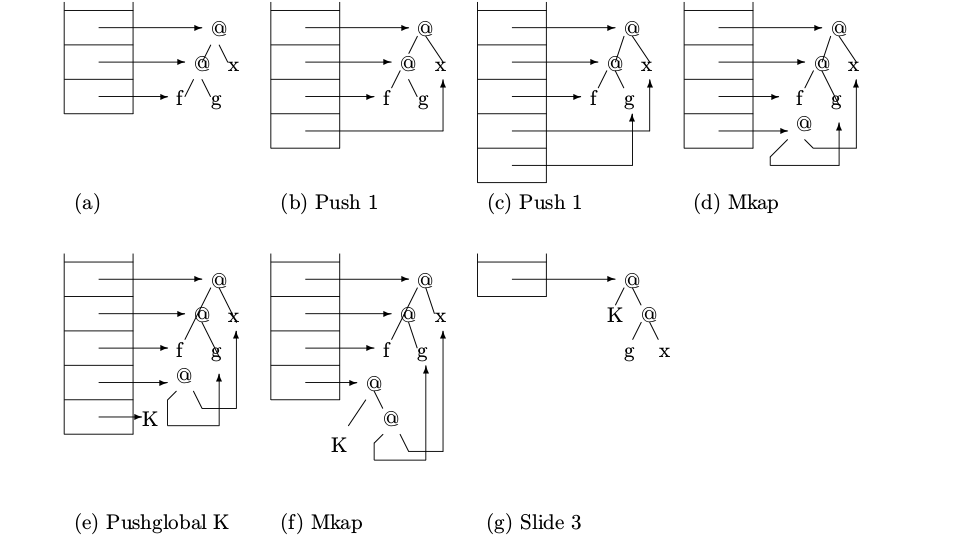
\includegraphics[scale=0.35]{primerGmasine.png}
		\caption{Vizuelni prikaz izvršavanja k\^ oda.}
		\label{fig:primerGmasine}
	\end{figure}

\end{frame}

\section{Zaključak}
\begin{frame}{Zaključak}
	
\end{frame}


\subsection{Literatura}
\begin{frame}{Literatura}
	
\end{frame}

\begin{frame}
	Hvala na pažnji!
\end{frame}
	
	
\end{document}